\section{Aufbau}

\subsection{Architektur}
\begin{figure}[htbp]
\centering
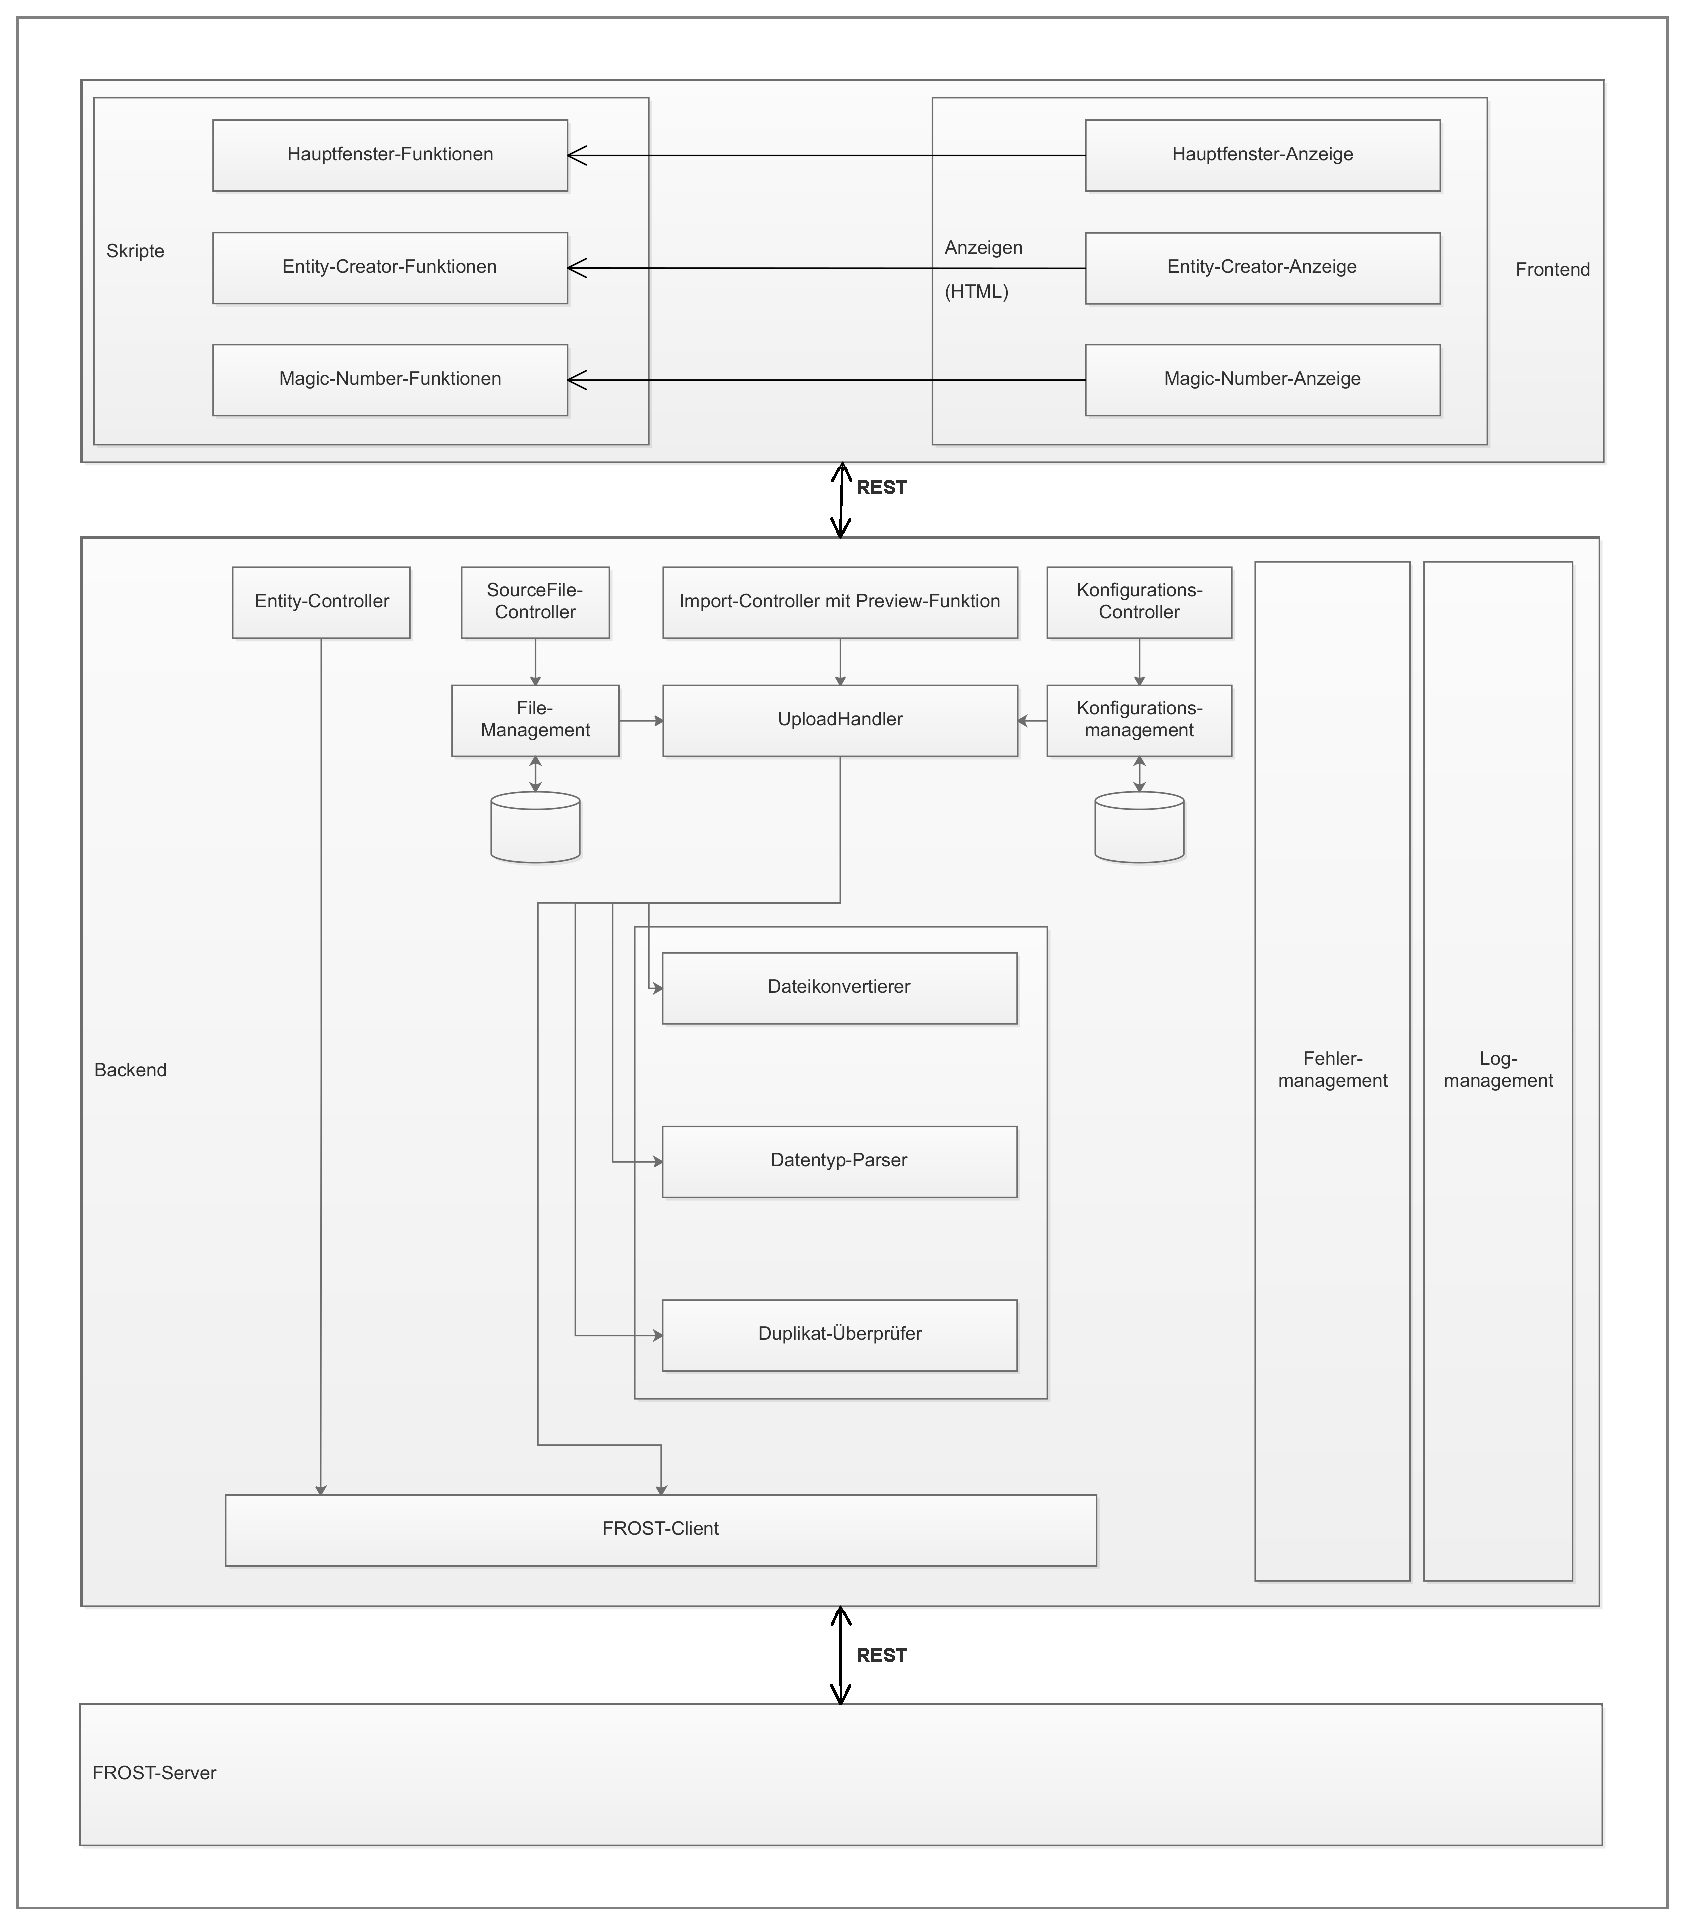
\includegraphics[scale=0.44]{uml/eps/architektur.eps}
\caption{\label{fig:architektur} Architekturmodell}
\end{figure}
\noindent Die Grobarchitektur der Software besteht aus einem Frontend, einem Backend und einem zugrundeliegenden FROST-Server.\\
 Das Frontend umfasst dabei vorwiegend die Darstellung der Webseite, während im Backend die Verarbeitung der Daten von der Webseite, die auf den FROST-Server geladen werden sollen, stattfindet. \\
 Eine nähere Beschreibung der Komponenten erfolgt hier:

\paragraph{Frontend}
Die Webseite wird mit einer Model-View-Controller-Architektur (MVC) modelliert.\\
Zum Einen stehen Skript-Klassen auf der Webseite zur Verfügung, die verschiedene Funtkionen realisieren und deren Daten speichern.
Zum Anderen gibt es Anzeige-Klassen die eine interaktive graphische Oberfläche zu diesen Funktionen bereitstellen.Dabei existiert für jede Skript-Klasse genau eine Anzeigeklasse.

\paragraph{Backend}
Das Backend ist zentraler Bestandteil der Software und enthält die Anwendungslogik.\\
Für die Kommunikation mit der Webseite stehen die Controller zur Verfügung.\\
Diese sind dafür zuständig Anfragen anzunehmen, zu überprüfen und an die passenden internen Komponenten weiterzugeben, sowie das Ergebnis passend aufzubereiten.\\

\noindent Im Konfigurationsmanagement werden Konfigurationen, die vom Benutzer über die GUI erstellt wurden, gespeichert, geladen und für andere Komponenten zur Verfügung gestellt.\\

\noindent Die Hauptfunktionalität der Software, das Hochladen von Daten auf den FROST-Server, läuft über die UploadHandler-Komponente.\\
Diese kann zur Verarbeitung der Daten auf andere Komponenten wie das Konfigurations- und das File-Management, die Konvertierung in ein internes Datenformat und das Erstellen der Observations (der Messwerte) zugreifen.\\
Mit der Duplikatsüberprüfung kann für eine gegebene Observation überprüft werden, ob diese schon auf dem Server existiert.\\
Neben dem Hochladen der Daten lässt sich über die Preview-Komponente auch das Anwenden der bestehenden Konfiguration auf die Daten der Quelldatei ansehen.\\
Sie muss im Gegensatz zum wirklichen Hochladen jedoch keine Observations auf dem FROST-Server erstellen.\\

\noindent Fehler und Logmanagement sind von allen Klassen aus ansprechbar und halten aufgetretene Fehler oder Benachrichtigungen für den User fest.

\noindent Zusätzlich besteht für die Controller noch Zugriff auf Komponenten zur Erstellung von Entities bzw. Abfragen von bestehenden Entities auf dem FROST-Server.\\
Sämtliche Kommunikation mit dem FROST-Server läuft dabei über den FROST-Client, einer existierenden Bibliothek zur Vereinfachung der Kommunikation mit dem FROST-Server.\\
Außerdem gibt es noch Komponenten zur Fehlerbehandlung und dem Erstellen eines Logs.

\paragraph{FROST-Server}
Der FROST-Server ist die Komponente, auf den die vom Nutzer gesammelten Daten übertragen werden.\\
Die Kommunikation mit dem Server findet durch den FROST-Client als Schnittstelle statt.\\
Der FROST-Client ist nicht Teil des Projekts, sondern wird als gegeben angenommen.

\clearpage
\subsection{Klassendiagramm}

\begin{figure}[!h]
\centering
\includegraphics[angle =90, scale=0.13]{Klassendiagramm/klassendiagramm.eps}
\caption{Klassendiagramm (siehe \nameref{anh} für größere Ansicht)}
\end{figure}